\documentclass[12pt, oneside]{extbook} % the document type needs to be change
\usepackage{geometry}
\usepackage{listings}
\usepackage{graphicx}
\usepackage[utf8]{inputenc}
\usepackage[T1]{fontenc}
\usepackage[italian]{babel}

\geometry{
    top = 1.5cm,
    bottom = 1.5cm,
    left = 2cm,
    right=2cm,
}

\begin{document}
\chapter{Blocco 3: Ethernet LAN security}
\section{Ethernet LAN recap}
Ethernet è una tecnologia di livello 2, il primo standard open e multi-vendor nato nel 1976.
\\L'802 è una famiglia di standard dell'IEEE, fra di essi ci sono diversi gruppi di lavoro e quello che si occupa di Ethernet è 802.3 e quindi si parla di questi standard, in quanto Ethernet era il nome commerciale.
\\La trama Ethernet originale ha un header molto snello, c'è il campo type / length che può essere due campi differenti a seconda della situazione, i campi sempre presenti sono:
\begin{itemize}
    \item Preambolo;
    \item indirizzo sorgente e destinazione;
    \item data;
    \item type/preamble;
    \item FCS;
\end{itemize}
(altri campi nelle versioni SNAP ed original).
\\Anche in questo caso è tutto in chiaro, quindi ci sono gli stessi problemi visti per IP.
\\Gli indirizzi MAC sono a 48 bit, dove i primi due bit hanno significato particolare, anche in base al valore

\subsection{Hub e Switch}
La differenza fondamentale fra gli strumenti sta in come viene effettuato il forwarding:
\begin{itemize}
    \item un hub è uno strumento che forwarda pacchetti verso tutti; 
    \item uno switch ha un forwading database, ovvero una struttura dati che associa MAC alle porte.
    \\Lo switch impara in automatico quale è il MAC dietro una certa porta.
    \\Il problema sta proprio nel fatto che lo switch impara in automatico il mapping.
\end{itemize}
Si usa l'algoritmo spanning three per evitare i loop, che si possono creare perché, per motivi di ridondanza, è possibile avere dei loop nella rete.

\subsection{Recap DHCP ed ARP}
Per operare al di sopra di Ethernet, IPv4 usa ARP e DHCP mentre IPv6 usa NDP, protocollo simile.
\\NDP non è sicuro, ma c'è un protocollo per renderlo sicuro e lo stesso protocollo è stato progettato già pensando alla sicurezza.
\\Anche nel caso di DHCP, usato per ottenere un IP, abbiamo gli stessi problemi detti sopra.\\
ARP è un protocollo semplice di richiesta/risposta:
\begin{itemize}
    \item le richieste vengono mandate broadcast
    \item le risposte arrivano invece in unicast
\end{itemize}
il pacchetto viene incapsulato nella trama ethernet e sfrutta dest e src per richiesta e risposta.
\\Per evitare di rifare ogni volta una richiesta per lo stesso indirizzo IP, ARP mantiene una cache di risoluzioni già effettuate, che dopo un certo TTL vengono buttate via.

\section{Ethernet LAN vulnerabilities}
Quali sono le possibili contro-misure per difendersi dai threats.
\\I problemi di Ethernet sono dovuti al fatto che per natura si auto-configura e siccome è possibile avere accesso a qualunque trama Ethernet, l'attaccante può:
\begin{itemize}
    \item imparare qualcosa sulla topologia della rete
    \item avere accesso agli switch
    \item eavesdropping
    \item etc..
\end{itemize}

Vediamo alcune categorie di problemi
\subsection{Network and system access}
Come è possibile ottenere accesso ad un Ethernet segment:
\begin{itemize}
    \item unioni non autorizzate:
    \begin{itemize}
        \item tramite accesso fisico allo switch, se la porta è attiva
        \item accedere ad una socket a muro
        \item rimuovere il cavo ad un PC e metterlo in un altro
        \item inserire uno switch fra il PC esistente e la socket
    \end{itemize}
    \item Espansioni della rete non autorizzate: l'architettura ethernet permette agli utenti di espandere la rete installando i propri switch o WAP e che quindi permette ad altri utenti di entrare nella rete;
    \item Accesso in maniera remota (VLAN join): se uno switch ascolta con un protocollo di gestione di VLAN, un host può far finta di essere uno switch ed entrare in tutte le VLANs 
    \item probe della rete per scoprire informazioni, come ad esempio usare nmap.
\end{itemize}

Altri modi:
\begin{itemize}
    \item break-ins: un attaccante può usare la rete Ethernet come mezzo di attacco verso altri host e switches della rete.
    \\Questi attacchi tipicamente hanno come target vulnerabilità nei livelli più alti dello stack di rete;
    \item switch control: uno switch che ha password di default o non la ha e la password può essere resettata fisicamente.
    \\Se si ottiene il controllo di uno switch si possono fare varie cose, ad esempio se lo switch gira su cumulus Linux
\end{itemize}

Una volta che si è ottenuto l'accesso alla rete, si può fare lo sniffing del traffico di rete.
\\Oggi non è più vero che la trama arriva a tutti e che sono tutti connessi, ma se c'è la possibilità di intercettare fisicamente il pacchetto allora è possibile fare un MiTM etc...
\\Il problema è anche nella procedura di learning dello switch il MAC non è autenticato, quindi mandando una trama con un MAC reale allo swtich, viene ingannato nel pensare che il MAC è dietro una porta sbagliata.
\\Quindi l'attaccante può redirigere il traffico trasmesso dalla vittima verso se stesso, anche se è più che altro teorico perché anche la vittima manda messaggi.
\\Si può generare un pacchetto con un indirizzo falso, o anche intercettare un pacchetto e cambiarlo in quanto anche a livello 2 non c'è integrity check o HMAC tag.
\\Per cambiare il MAC, ci sono vari modi:
\begin{itemize}
    \item cambiare il MAC della NIC (comando Linux)
    \item usare raw socket programming
    \item in-kernel programming
\end{itemize}
Per intercettare il pacchetto, basta mettere l'interfaccia di rete in modalità promiscua per ricevere tutto il traffico anche non diretto a me, così da poter cambiare il MAC.

\subsection{Traffic integrity}
Anche qui ci sono diversi attacchi:
\begin{itemize}
    \item MAC flooding: l'idea è di inondare lo switch con un grande numero di trame con diversi indirizzi MAC per saturare la memoria dello switch in modo da far si che tutti i pacchetti siano inviati verso tutte le porte in broadcast;
    \item ARP and DHCP poisoning: si può fare ARP poisoning (vedi sopra) ma anche facendo poisoning di DHCP facendo credere di essere il server, spoofando tutto lo scambio DHCP.
    \\Nell'ARP poisoning si avvelena tutta la ARP cache, che è usata per memorizzare risultati di precedenti ARP request per evitare di rifarle ogni volta (ogni riga ha comunque un TTL).
    \\È sempre possibile configurare la cache ARP in maniera statica.
    \\Le ARP gratuite sono utili per vari motivi, non solo pericolosi;
    \item MiTM: È possibile fare un MiTM: ho un PC ed un default gateway, mando una ARP response (op code 2) col MAC della vittima al default gateway ed una ARP response col MAC del default gateway alla vittima.
    \\(N.B:ARP non è stato progettato specificamente per mappare IP-MAC, ma per associare un indirizzo di layer 3 ad uno di layer 2).
    \item Session hijack: a livello 2, Ethernet non ha conoscenza della sessione, è come IP.
    \\Non c'è relazione fra pacchetti inviati in sequenza, e questo è un'altra vulnerabilità.
    \\È possibile dirottare una sessione e iniziare a trasmetterli in una sessione già stabilita, perché Ethernet non ha protezioni per questo.
    \item Denial of service: l'obiettivo è quello di negare il servizio, si può fare nel layer Ethernet.
    \\È possibile esaurire le risorse di una macchina, cercare di far crashare lo switch ma anche farlo a livello di protocollo.
    \\STP (Spannign Three Protocol) permette di gestire grandi topologie di rete, con molti switch e link ridondanti, quindi loop fisici.
    \\Con STP si disabilita la porta che causa il loop, ma anche STP non  autenticato e si può far credere di essere uno switch.
\end{itemize}

\subsection{Contromisure}
Per risolvere i problemi, è stato deciso che tutte le trame Ethernet vengano marcate come non sicure.
\\Per farlo è necessario metterlo in un dominio protetto, ovvero protezioni perimetrali come il firewall etc...
\\Altrimenti, è possibile usare soluzioni crittografiche, in ogni caso ci sono 4 categorie di contromisure:
\begin{itemize}
    \item router based security: se si può rimpiazzare uno switch con un router, si risolvono molti problemi.
    \\Un IP router messo fra tutti i nodi, non c'è un singolo dominio di broadcast, che è interrotto perché il router non forwarda i pacchetti in broadcast.
    \\In questo modo si risolvono ARP, STP, MAC table based attacks. (Si possono avere dei singoli dominii di broadcast usando le VLAN.)
    \item access control: se non si può sostituire con un router, si può comunque controllare chi accede alla rete in differenti modi.
    \\Per farlo, uno dei modi è usare il protocollo 802.1X port authentication: l'idea è che la porta di uno switch è aperta solo se il client \texttt{s} è autenticato correttamente verso un'altra entità, che è l'authentication server.
    \\Un altro modo è usare le ACL (Access Control List).
    \\Il problema rimane, perché i MAC sono comunque spoofabili e quindi i pacchetti non sono comunque protetti e possono essere forgiati a piacere
\end{itemize}
\subsubsection{Central managed LAN}
Sarebbe utile avere una entità centrale per poter garantire l'accesso in rete ed i progetti sono per lo più di ricerca:
\begin{itemize}
    \item SANE: ogni client ha del software e prima di poter comunicare con lo switch deve mandare una richiesta al punto centrale
    \item Ethane: i client non devono avere nessun software sull' IP/TCP stack: per ogni pacchetto, è lo switch a mandare i pacchetti alla entità centrale ed è quella che dice se i pacchetti vengono accettati oppure droppati.
    \\È simile al concetto dell SDN: il controllo è separato dai dati, il data plane è staccato dal control plane.
    \\L'idea è che il software procede molto più velocemente dei protocolli di rete, perché è più facile e ci sono interfacce di programmazione ben definite.
    \\Non è facile invece aggiornare un protocollo e come questo viene implementato: l'hardware è comunque più veloce del software in quanto è specializzato mentre per il software c'è un grande overhead dovuto al SO, al kernel etc... mentre l'hardware è dedicato.
\end{itemize}

\paragraph{OpenFlow} una delle prime implementazioni di SDN, lo stack di networking è diviso in data plane e control plane.
\\OpenFlow definisce come è fatto il data plane ed anche il protocollo per iniettare il codice di configurazione nel control flow.
\\Inoltre, OpenFlow è fatto da una pipeline di flow table, per cui se ho un miss nella tabella di routing il controllo passa al control plane che è fatto nel linguaggio preferito.
\\Quindi, dopo averlo processato, viene rimandato allo switch con un comando (regola) che dice come trattare tutti i successivi pacchetti dallo stesso IP.
\\Non è stata progettata per essere sicura ma il processamento: una volta che ho imparato dal primo pacchetto cosa fare, tutti gli altri sono processati velocemente.
\\Non è scalabile, in quanto il control plane centralizzato riceve tutti i pacchetti nuovi e diventa il collo di bottiglia.
\\Viene però centralizzata la decisione su cosa fare per i pacchetti, come dicevamo sopra.

\subsubsection{Sicurezza dei protocolli: MACsec}
Perché non applicare un approccio crittografico per la sicurezza al livello 2: abbiamo TLS ed IPSec per il 5 ed il 3.
\\Abbiamo MACsec, che è come l'IPsec per Ethernet.
\\Definisco il parametro dell'associazione, non sono obbligatori, ma abbiamo:
    \begin{itemize}
        \item confidenzialità
        \item integrità
        \item anti-replay
    \end{itemize}
È più simile ad IPsec, in quanto TLS è all-in-one: definisce sia come implemetare le sessioni sicure che come fare l'handshake.
\\Mentre MACsec non definisce la fase di negoziazione, che è fatta con un protcollo apposito.
\\L'header di MACsec può avere come opzionali il TAG per l'autenticazione e la parte di encryption.
\\Serve anche il sequence number perché Ethernet non è reliable, a differenza di TLS che poggia su TCP.
\\Come in IPsec, la Security Association che viene creata è mono-direzionale e quindi va ogni volta creata in entrambe i versi della comunicazione.
\subsubsection{Security monitoring}
Ci può essere controllo sull'accesso alla rete, ma non si può essere sicuri che i client non siano malevoli. Si può quindi monitorare il traffico con un Ethernet firewall ma non ha senso fare la differenza dei firewall ai diversi livelli.
\\Altrimenti ci sono IDS e Prevention System, le implementazioni più importanti open sono source

\section{IPv6 SEcure Neighbour Discovery}

\subsection{IPv6 neighbour discovery}
La prima motivazione per implementare IPv6 è che l'IPv4 ha indirizzi troppo corti che sono finiti, ma le altre motivazioni riguardano il neighbour discovery.
\\In IPv4 ci sono vari protocolli come DHCP, ICMP, ARP che sono di controllo e gestione, in IPv6 è tutto unificato e fatto da ICMPv6 in maniera migliore e più chiara.
\\La neighbour discovery viene fatta per capire il MAC associato ad un IPv6, o chi è il deafult gateway etc... e può essere fatto tutto con IPv6 neighbour discovery.
\\Non è un meccanismo in se ma un protocollo che definisce dei messaggi, con cui si può
    \begin{itemize}
        \item scoprire un gateway
        \item fare redirection
        \item etc...
    \end{itemize}
I messaggi base definiti da ICMPv6 per il protocollo di neighbour discovery sono i seguenti
    \begin{itemize}
        \item Router Solicitation
        \item Router Advertisment
        \item Neighbour Solicitation
        \item Neighbour Advertisment
        \item Redirect Message
    \end{itemize}
Ogni combinazione di messaggi viene usata per fare una delle azioni che in IPv4 viene fatta con un protocollo apposito
\subsubsection{Neighbour solicitation e Advertisment}
In questo caso, un nodo può usare degli indirizzi speciali:
    \begin{itemize}
        \item multicast verso tutti: indirizzo con prefisso (FF02::1, destinazione) (:: = 0:0...)
        \item Multicast verso tutti i router: (FFO2::1, dest)
        \item indirizzo multicast per fare solicitation
    \end{itemize}
Per fare Address Resolution si manda il neighbour solicitation e si riceve il messaggio di risposta per poter risolvere il MAC associato ad un IPv6.
\\Anche in questo caso, non ci sono concetti di sicurezza 
    \begin{itemize}
    \item DoS: per configurare un IPv6 è possibile fare una cosa nuova, ovvero senza DHCPv6 perché la neighbour discovery è possibile scoprire chi sono i router, capire il prefisso della rete e serve solo la parte host dell'indirizzo.
    \\Siccome gli indirizzi sono molto lunghi, è possibile auto-configurare un IP che non collida con quello di qualche altro nodo della rete.
    \\Ora, bisogna cercare se c'è duplicazione dell'IPv6.
    \\Se si vuole fare DoS, si intercettano i messaggi di richiesta duplicati e si dice che l'host esiste già
\end{itemize}
ma la crittografia è implementata come estensione al protocollo con la Secure Neighbour Discovery: si usano 4 nuovi messaggi
    \begin{itemize}
        \item CGA: possiamo fare il binding fra IP address con un dispositivo senza una CA?
        \\Sì, un IP generato crittograficamente: abbiamo una chiave pubblica, ogni volta che mandiamo un messaggio lo firmiamo con la chiave privata e chiunque riceve può verificare che nessuno  sta spoofando quell'IP.
        \\I 64 bit più signifcativi sono il prefisso della rete e i restanti di host, ha anche dei parametri di sicurezza per pararsi da bruteforce attacks.
        \\La struttura dati associata alla CGA è la seguente:\\
            \begin{figure}[h!]
            \centering
            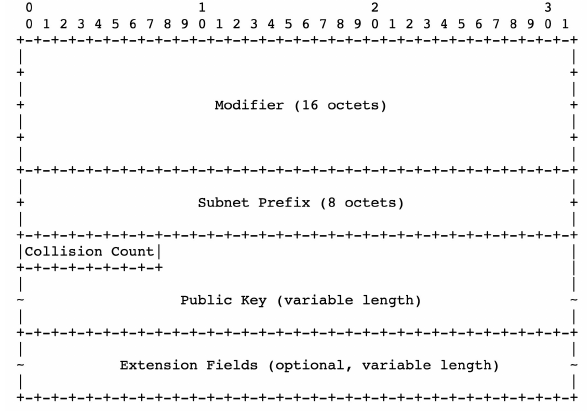
\includegraphics[scale=0.4]{../../immagini/cga_struct.png}
        \end{figure}\\\\
        La generazione avviene a partire dalla struttura dati della CGA: l'algoritmo scegli un modificatore random, seleziona un valore sicuro e mette il collision number a 0.
        \\Si fa SHA-1 e si prendono 112 bit, si verifica poi che 16*(sec leftmost Hash2 bits) sia 0, per poter essere robusti a bruteforcing.
        \\Se il prodotto non fa 0, si riparte e se dopo la generazione del CGA c'è una collisione, ovvero un IP duplicato, va incrementato il counter della collision.
        \\Siccome non è spiegato come controllarlo ma va fatto, ci sono vulnerabilità associate e quindi il controllo va protetto.
        \\Si continua poi con la generazione:\\
            \begin{figure}[h!]
                \centering
                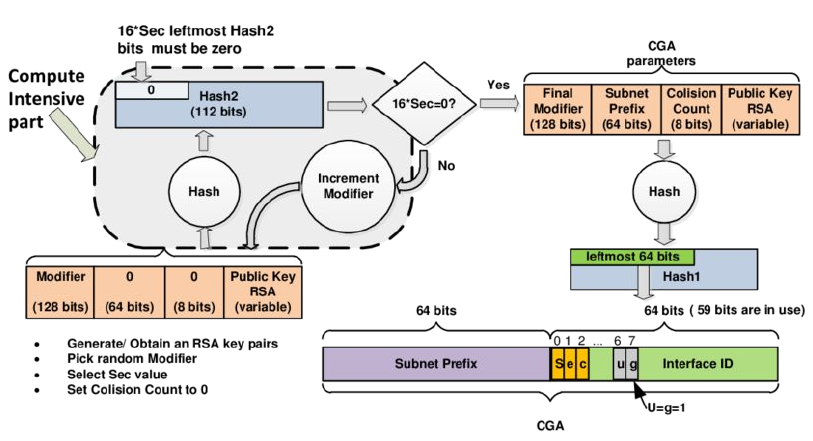
\includegraphics[scale=0.5]{../../immagini/cga_computation}
            \end{figure}\\\\
        La cosa importante è che ci sia una chiave pubblica legata ad un IP address, in modo ad non avere una CA per ogni nodo che entra in una rete e quindi non sia richiesto un certificato.
        \\È vero che si può generare una CGA propria se si è un attaccante, ma le CGA non sono usate per fare authorization, quindi non è possibile spoofare un address perché dovrebbe trovare una collisione nell'hash function (che è crittografica) ed inoltre non si può generare la chiave privata associata alla chiave pubblica. Per questo, ci sono dei tipi di attacco differenti.
        \\ C'è una opzione della CGA per verificare la firma dopo aver verificato la CGA: se uno dei due controlli fallisce, il pacchetto non è valido
    \item RSA signature: opzionale, metto una firma fatta con RSA nel messaggio. Se è un router, abbiamo la chiave pubblica del router, altrimenti quella pubblica del client associata all'IP
\item Nonce e Timestamp
\end{itemize}
\subsection{Router Authorization}
Otteniamo un messaggio di Router "?" che è autenticato dal fatto che il router ha un certificato dato da una CA, se l'host ha la chiave della CA può verificare che il messaggio è effettivamente autentico.

\subsection{Conclusioni}
Mettendo tutto insieme, ICMPv6:
    \begin{enumerate}
        \item il nodo 1 vuole scoprire un certo MAC e quindi manda un messaggio di sollecitazione. Avrà una sua chiave pubblica (slides)
        \item dopo tutto il pippone di roba, si firma tutto il pacchetto con la chiave privata usando l'algoritmo e si appende l'opzione della firma RSA e viene mandato il pacchetto
    \end{enumerate}
Il receiver:
    \begin{enumerate}
        \item Controllare i parametri della CGA ed l'indirizzo IPv6 sorgente, calcolando lo SHA-1 dai parametri CGA e verificando con ipv6.src.
        \\Se il Sec = 0, va bene altrimenti controlla anche Hash2
        \item Controllare la nonce
        \item Controllare la signature
\end{enumerate}
Si procede con i passi scritti sulle slides\\ Le conclusioni:
\begin{itemize}
    \item il protocollo SEND garantisce che:
        \begin{itemize}
            \item l'NA non venga spoofato, ovvero sia mandato dal legittimo proprietario del CGA nel pacchetto, ovvero sia mandato dal legittimo proprietario del CGA nel pacchetto
            \item l'NA non sia stato modificato
            \item l'NA non sia stato replayed 
        \end{itemize}
\end{itemize}
Ha però diversi limiti fra cui computazionali, di implementazione, di deployment, di sicurezza che potrebbero far si di essere vulnerabili a determinati attacchi.

\end{document}
